%%%%%%%% ICML 2019 EXAMPLE LATEX SUBMISSION FILE %%%%%%%%%%%%%%%%%

\documentclass{article}

% Recommended, but optional, packages for figures and better typesetting:
\usepackage{microtype}
\usepackage{graphicx}
\usepackage{subfigure}
\usepackage{booktabs} % for professional tables

% hyperref makes hyperlinks in the resulting PDF.
% If your build breaks (sometimes temporarily if a hyperlink spans a page)
% please comment out the following usepackage line and replace
% \usepackage{icml2019} with \usepackage[nohyperref]{icml2019} above.
\usepackage{hyperref}



% Attempt to make hyperref and algorithmic work together better:
\newcommand{\theHalgorithm}{\arabic{algorithm}}

% Use the following line for the initial blind version submitted for review:
%\usepackage{icml2019}

\usepackage[utf8x]{inputenc}

% If accepted, instead use the following line for the camera-ready submission:
\usepackage[accepted]{icml2019}

% The \icmltitle you define below is probably too long as a header.
% Therefore, a short form for the running title is supplied here:
\icmltitlerunning{Training Data Poisoning for Imperfect Information Games}

\begin{document}

\twocolumn[
\icmltitle{Training Data Poisoning for Imperfect Information Games}

% It is OKAY to include author information, even for blind
% submissions: the style file will automatically remove it for you
% unless you've provided the [accepted] option to the icml2019
% package.

% List of affiliations: The first argument should be a (short)
% identifier you will use later to specify author affiliations
% Academic affiliations should list Department, University, City, Region, Country
% Industry affiliations should list Company, City, Region, Country

% You can specify symbols, otherwise they are numbered in order.
% Ideally, you should not use this facility. Affiliations will be numbered
\icmlsetsymbol{equal}{*}

\begin{icmlauthorlist}
\icmlauthor{Guy Aridor}{cuecon}
\icmlauthor{Natania Wolansky}{cu}
\icmlauthor{Jisha Jacob}{cu}
\icmlauthor{Iddo Drori}{cu}
\end{icmlauthorlist}

\icmlaffiliation{cuecon}{Department of Economics, Columbia University} \\
\icmlaffiliation{cu}{Department of Computer Science, Columbia University}


\icmlcorrespondingauthor{Guy Aridor}{ga2449@columbia.edu}

% You may provide any keywords that you
% find helpful for describing your paper; these are used to populate
% the "keywords" metadata in the PDF but will not be shown in the document
\icmlkeywords{Machine Learning, Imperfect Information Games}

\vskip 0.3in
]

% this must go after the closing bracket ] following \twocolumn[ ...

% This command actually creates the footnote in the first column
% listing the affiliations and the copyright notice.
% The command takes one argument, which is text to display at the start of the footnote.
% The \icmlEqualContribution command is standard text for equal contribution.
% Remove it (just {}) if you do not need this facility.

\printAffiliationsAndNotice{}  % leave blank if no need to mention equal contribution
%\printAffiliationsAndNotice{\icmlEqualContribution} % otherwise use the standard text.

\begin{abstract}
This work explores how simple strategies in the game of Leduc Hold'em can be used to beat a sophisticated poker AI, DeepStack. We first analyze, under unbiased training, how significantly DeepStack outperforms most traditional poker-playing strategy profiles employed by humans. We then consider the ability of an opponent to bias the training phase such that DeepStack is optimized to play against a particular strategy profile. Finally, by allowing for this biasing, we show that DeepStack can be defeated by a subset of strategy profiles if the player can change their strategy post-training. While DeepStack achieves nearly super-human performance, we conclude that DeepStack is susceptible to training poisoning.
\end{abstract}

\section{Introduction}
\label{Introduction}

Most of the recent breakthrough work in artificial intelligence has been in developing agents that can play difficult multi-agent games such as chess, shogi, Go, or poker at super-human levels. These agents have been developed leveraging large amounts of computational power as well as utilizing advances in deep learning and reinforcement learning. However, are these agents susceptible to defeat by strategic agents with little computational power with the ability to bias training? In real world chess and poker tournaments, grandmasters and expert players often use strategies of deception in practice rounds and early rounds of the tournament to confuse their opponents about the strategies they employ later on. In this paper we look at the consequences of not taking this into account when training against players who may have adversarial intentions. While adversarial examples check the robustness of neural networks by testing the generalization capability of the network with examples which confuse the network into mis-classification, this work explores the training process rather than testing time, namely training data poisoning. 

We are interested in asking how (and if) strategic agents interacting with these systems can manipulate such systems in order to at least improve a simple agent's relative performance, or better yet, defeat such systems. In this work we explore this in the case of Leduc poker, utilizing an existing, state-of-the-art implementation that plays at super-human levels. 
We allow an agent to play according to a particular ``profile" of strategies in the training phase and then switch profiles during ``real" play and explore if this can allow the individual to substantially improve performance and potentially beat the AI agent.

We utilize recent breakthrough work in playing imperfect information games \cite{moravvcik2017deepstack}, \cite{brown2018depth} that achieve super-human results in game-play by optimizing towards Nash-equilibrium strategies in Leduc Hold'em and Head-Up No-Limit Poker. However, there is considerable evidence that humans in games deviate from rationality substantially \cite{goeree2001ten} exhibiting changes in risk-tolerance over the course of play \cite{eil2014staying}. On the one hand, since Heads-Up No-Limit Poker is a two-player zero-sum game, this almost ensures that deviations from rational play will lead to defeat (on average) by agents trained on optimizing towards Nash-equilibrium strategies. On the other hand, it also leaves on the table the fact that there may be better strategies than playing Nash Equilibrium that may yield a higher average payoff by exploiting human irrationality and behavioral biases in the absence of a human player's ability to compute Nash Equilibrium. This leaves open the possibility that, in some cases, it may be better to optimize towards these strategies instead of the Nash Equilibrium strategy. Doing so, however, is not without its risks as optimizing towards strategies that exploit the weaknesses of a particular profile may leave the agent susceptible to having these be exploited if the human player switches their player profile.

\indent In this work we suppose that a human player selects from a class of profiles that are feasible but that all have some inherent bias that is common in human poker-playing. However, the player can strategically switch between profiles during training and during real game-play. We first document by how much the common player profiles that we identify lose, on average, against an unbiasedly trained implementation of DeepStack \cite{moravvcik2017deepstack}. Then, we bias the training of DeepStack using one of our player profiles and show that the performance of other player profiles substantially improves and, surprisingly in some cases, beats the biased DeepStack on average.

\section{Related Work}\label{sec:related}

\subsection{Counterfactual Regret Minimization}
Counterfactual regret minimization is a foundational approach to improve performance in imperfect information games. Additionally, two notable approaches have been explored to overcome the challenges of states lacking unique values. Recursive reasoning approaches to solve imperfect-information games have been explored since 2008. Counterfactual regret minimization (CFR) exploits the degree of incomplete information in an extensive game and uses self-play to recursively reason.

\indent Self-play enables an AI agent to adapt its playing strategy against itself over many iterations, leveraging "regrets" of prior decisions to inform future play. The AI agent's goal is to optimize its game tree traversal based on its opponent to converge on the Nash equilibrium. The limitation of this approach comes when dealing with larger game trees where such computation during play is too expensive. In these cases, abstraction is used to simplify the game which is then approximately solved via tabular CFR. Two types of abstractions have been historically employed -- information abstraction, where information sets are bundled, and action abstraction, where a subset of actions are removed from the game tree model.

\indent Recent work has explored an innovation on the tabular CFR approach that introduces Deep CFR, a form of CFR that uses function approximation with deep neural networks to approximate the tabular CFR behavior without the need for game abstraction \cite{brown2018deep}.

\begin{table*}[!b]
\small
\centering
{\begin{tabular}{|l|l|l|}
\hline
Player Profile & Type & Description \\
\hline\hline
Random & Probabilistic & Always plays a random, valid action \\
Rocks & Rules-based & Risk-averse player with strict folding logic. \\
Passive-Rocks & Rules-based & Risk-averse player with nuanced folding logic. \\
Mild Adaptive Rocks & Intelligent & Player that adjusts behavior based on success variance for state\\
Strong Adaptive Rocks & Intelligent & Player that adjusts behavior based on success variance for state\\
Always Calls & Rules-based & Player that always calls \\
Smart Bluffer & Intelligent & Risk-tolerant player that raises based on the probability of the opponent folding. \\
Random Bluffer & Probabilistic & Risk-tolerant player that randomly bluffs in play. \\
Always Raises & Rules-based & Maximally Risk-tolerant player who always raises by the maximum amount possible \\
\hline
\end{tabular}}
\caption{List of the irrational playing profiles explored.}
\label{tab:playerprofiles}
\end{table*}

\subsection{DeepStack \& Libratus}
AI DeepStack's technique modifies the definition of state into a joint belief state across all players \cite{moravvcik2017deepstack}, proving inferior to the top two HUNL Poker players. DeepStack's architecture consists of a standard feedforward neural network with seven fully connected hidden layers, each with 500 nodes and parametric rectified linear units (32) as output. This network is then embedded in another network imposing counterfactual regret minimization to satisfy the zero-sum property. Libratus approximates the optimal strategy for the earlier part of HUNL Poker and then approximates the best play in the latter parts of the game. This approach enabled Libratus to devise better strategies for particular subgames while fitting these strategies within the overarching blueprint. Libratus' architecture differentiates from DeepStack due to it's self-improver module that facilitates an open-loop to progressively learn from playing history.

\subsection{DeepStack-Leduc}
Extending the approach of \cite{brown2018depth}, Schmid et. al re-implemented the DeepStack AI agent for HUNL Leduc Hold'em. This adaptation to a simplified game laid the groundwork for rapidly exploring the performance impact of introducing irrationality in play.

\subsection{Adversarial Examples}
Our approach is very similar to the literature on adversarial examples (see \cite{yuan2017adversarial} for an overview), which attempts to construct inputs that can ``fool" otherwise well-behaved machine learning models. The consequences of the possibility of training data poisoning has been studied in several other methods. \cite{li2016data} looks at training poisoning in the context of collaborative filtering, \cite{biggio2012poisoning} in SVM, \cite{liu2017robust} in linear regression, \cite{alfeld2016data} in autoregressive models, \cite{xiao2015feature} in feature selection. \cite{steinhardt2017certified} studies defenses against training data poisoning.
To our knowledge we are the first to explore this in the context of imperfect information games and in particular with DeepStack. Our main focus is on whether a player can strategically manipulate the games DeepStack plays on in order to defeat DeepStack in ``real" gameplay by playing differing strategies in the training stages and the ``real" stages. We are not aware of an approach in the literature similar to this.

\section{Problem Formulation}
\subsection{Nash Equilibrium Strategy}

Most algorithms for learning how to play Leduc and HUNL attempt to approximate a Nash Equilibrium strategy. A Nash Equilibrium represents a profile of strategies in a game in which no player can improve her payoffs by changing to a different strategy. However, given the difficulty of approximating a Nash Equilibrium in these games, many players play non-optimal strategies. As a result, by learning from actual play it is likely that the strategy that eventually gets learned may not be the Nash Equilibrium strategy, but yet may produce better payoffs (on average) against the sub-optimal strategies of the opponent compared to the Nash Equilibrium strategy.

\subsection{Leduc Hold'em}
To explore semi-rational and psychologically manipulative playing agents, we use the simplified Poker game of Leduc Hold'em. When compared to HUNL, Leduc Hold'em has a smaller game tree and reduces playing time, drastically reducing time to learn.

\indent Leduc Hold’em is a two-player poker game with a six-card deck consisting of Jacks, Queens and Kings (two of each). The deck is shuffled prior to each hand and the game begins with a one-chip ante and a private card dealt to each player. An initial betting round transpires followed by the flop, where a single public card is shown. A second betting round transpires before the showdown where players reveal their private cards. The player with a pair wins the pot and in the case where neither does, the highest private card wins. If both players have a pair, then they split the pot.

\subsection{Limitations of Rationality in Poker}
In traditional poker, understanding your opponent's risk-tolerance and playing strategy is critical to winning. Common strategies in poker include bluffing, evaluating risk, and limiting exposure to exploitation. These are all computationally-simple attempts at a similar resolving process to what DeepStack simulates.

\section{Methodology}
Our approach explores rules-based, probabilistic and intelligent, semi-rational AI agents. We pit the agent against both an unbiased and biased trained DeepStack. There are four types of personalities in poker categorized based on their level of risk-tolerance and their level of aggression (i.e. Passive vs. Aggressive).

\subsection{Player Profiles Explored}

\indent While these basic four types (Tight-passive: The Rock, Tight-aggressive: The TAG, Loose-passive: The Calling Station, Loose-aggressive: The LAG) are well known, we expand our definitions with the understanding that there can be multiple types of risk-aversion, risk-tolerant, passive, and aggressive players \cite{teafilo2013}.

\indent Table \ref{tab:playerprofiles} outlines an initial list of player profiles explored in this work, with a focus on modeling risk-aversion and bluffing behaviors typically found in poker.  The players chosen represent a range of strategies that involve using different information estimated by a DeepStack-based player, as well as probabilistic and deterministic strategies.

\subsection{Risk-Averse Players}
Rocks represents a very risk-averse (i.e. "tight") personality type that folds in most cases when a high value card or potential pair does not exist. In the strategy space of Leduc Hold'em, this translates to playing only when the private card is a King. An example scenario of this player is found in Figure \ref{fig:short}. Passive Rocks will call or bet in some cases beyond the the highest value card. In the strategy space of Leduc Hold'em, this translates to playing hands that consist of a Queen or King. Both of these traditional risk-averse playing profiles are easily modeled using a rules-based approach.

\indent The Adaptive Rocks players use DeepStack's lookahead to determine which is the least risky play. They consider all actions they reasonably might take (actions that have more than 15\% probability according to DeepStack's estimation) and calculate the counterfactual value if each action is taken, estimating the variance of the value for that action over the possible opponent's hand. The Strong Adaptive Rocks player then deterministically chooses the action with the lowest variance. The Mild Adaptive Rocks player flips a coin to choose between the conservative, variance-minimizing move and the probabilistically-chosen rational move.

\subsection{Risk-Tolerant Players}
The above section explores the various conservative players implemented.  On the other side of the spectrum are players who are over-confident, bluffing more than would be rationally necessary. The Randomized Bluffer player spreads bluffs out randomly in play, regardless of the current value of the state of the game. This player bluffs by going all-in with 30\% probability if a raise is a valid move, and plays rationally (according to DeepStack's strategy) at all other times. 

\indent The Smart Bluffer player is a more intelligent agent that still over-bluffs but uses the counterfactual value of the opponent (in the game's current state) to determine whether she stands in a "good" or "bad" position relative to the opponent. This player (the Smart Bluffer) therefore takes the expected value of the opponent's counterfactual value of the game. If this expected value is below the opponent's value at the start of the hand (before cards are dealt), then the player is considered ``in a good state" and will raise liberally in a deterministic way. If not, she will play rationally according to DeepStack's strategy (this comparison to the value before cards are dealt is to deal with the natural difference in game value for P1 and P2 in Leduc and many other poker games).

\subsection{Control Players}
We also implement some players who use very simple, predictable strategies in order to compare our agents with more nuanced strategies. We implement two players, Always Call and Always Raise, who are somewhat self-explanatory. We also implement a truly random agent, who at each stage of the game chooses uniformly at random a valid action at that stage. This is in some sense the most "irrational" a player can get, and so is a good baseline for comparison.

\begin{figure*}[!b]
\begin{center}
\fbox{\rule{0pt}{0.5in}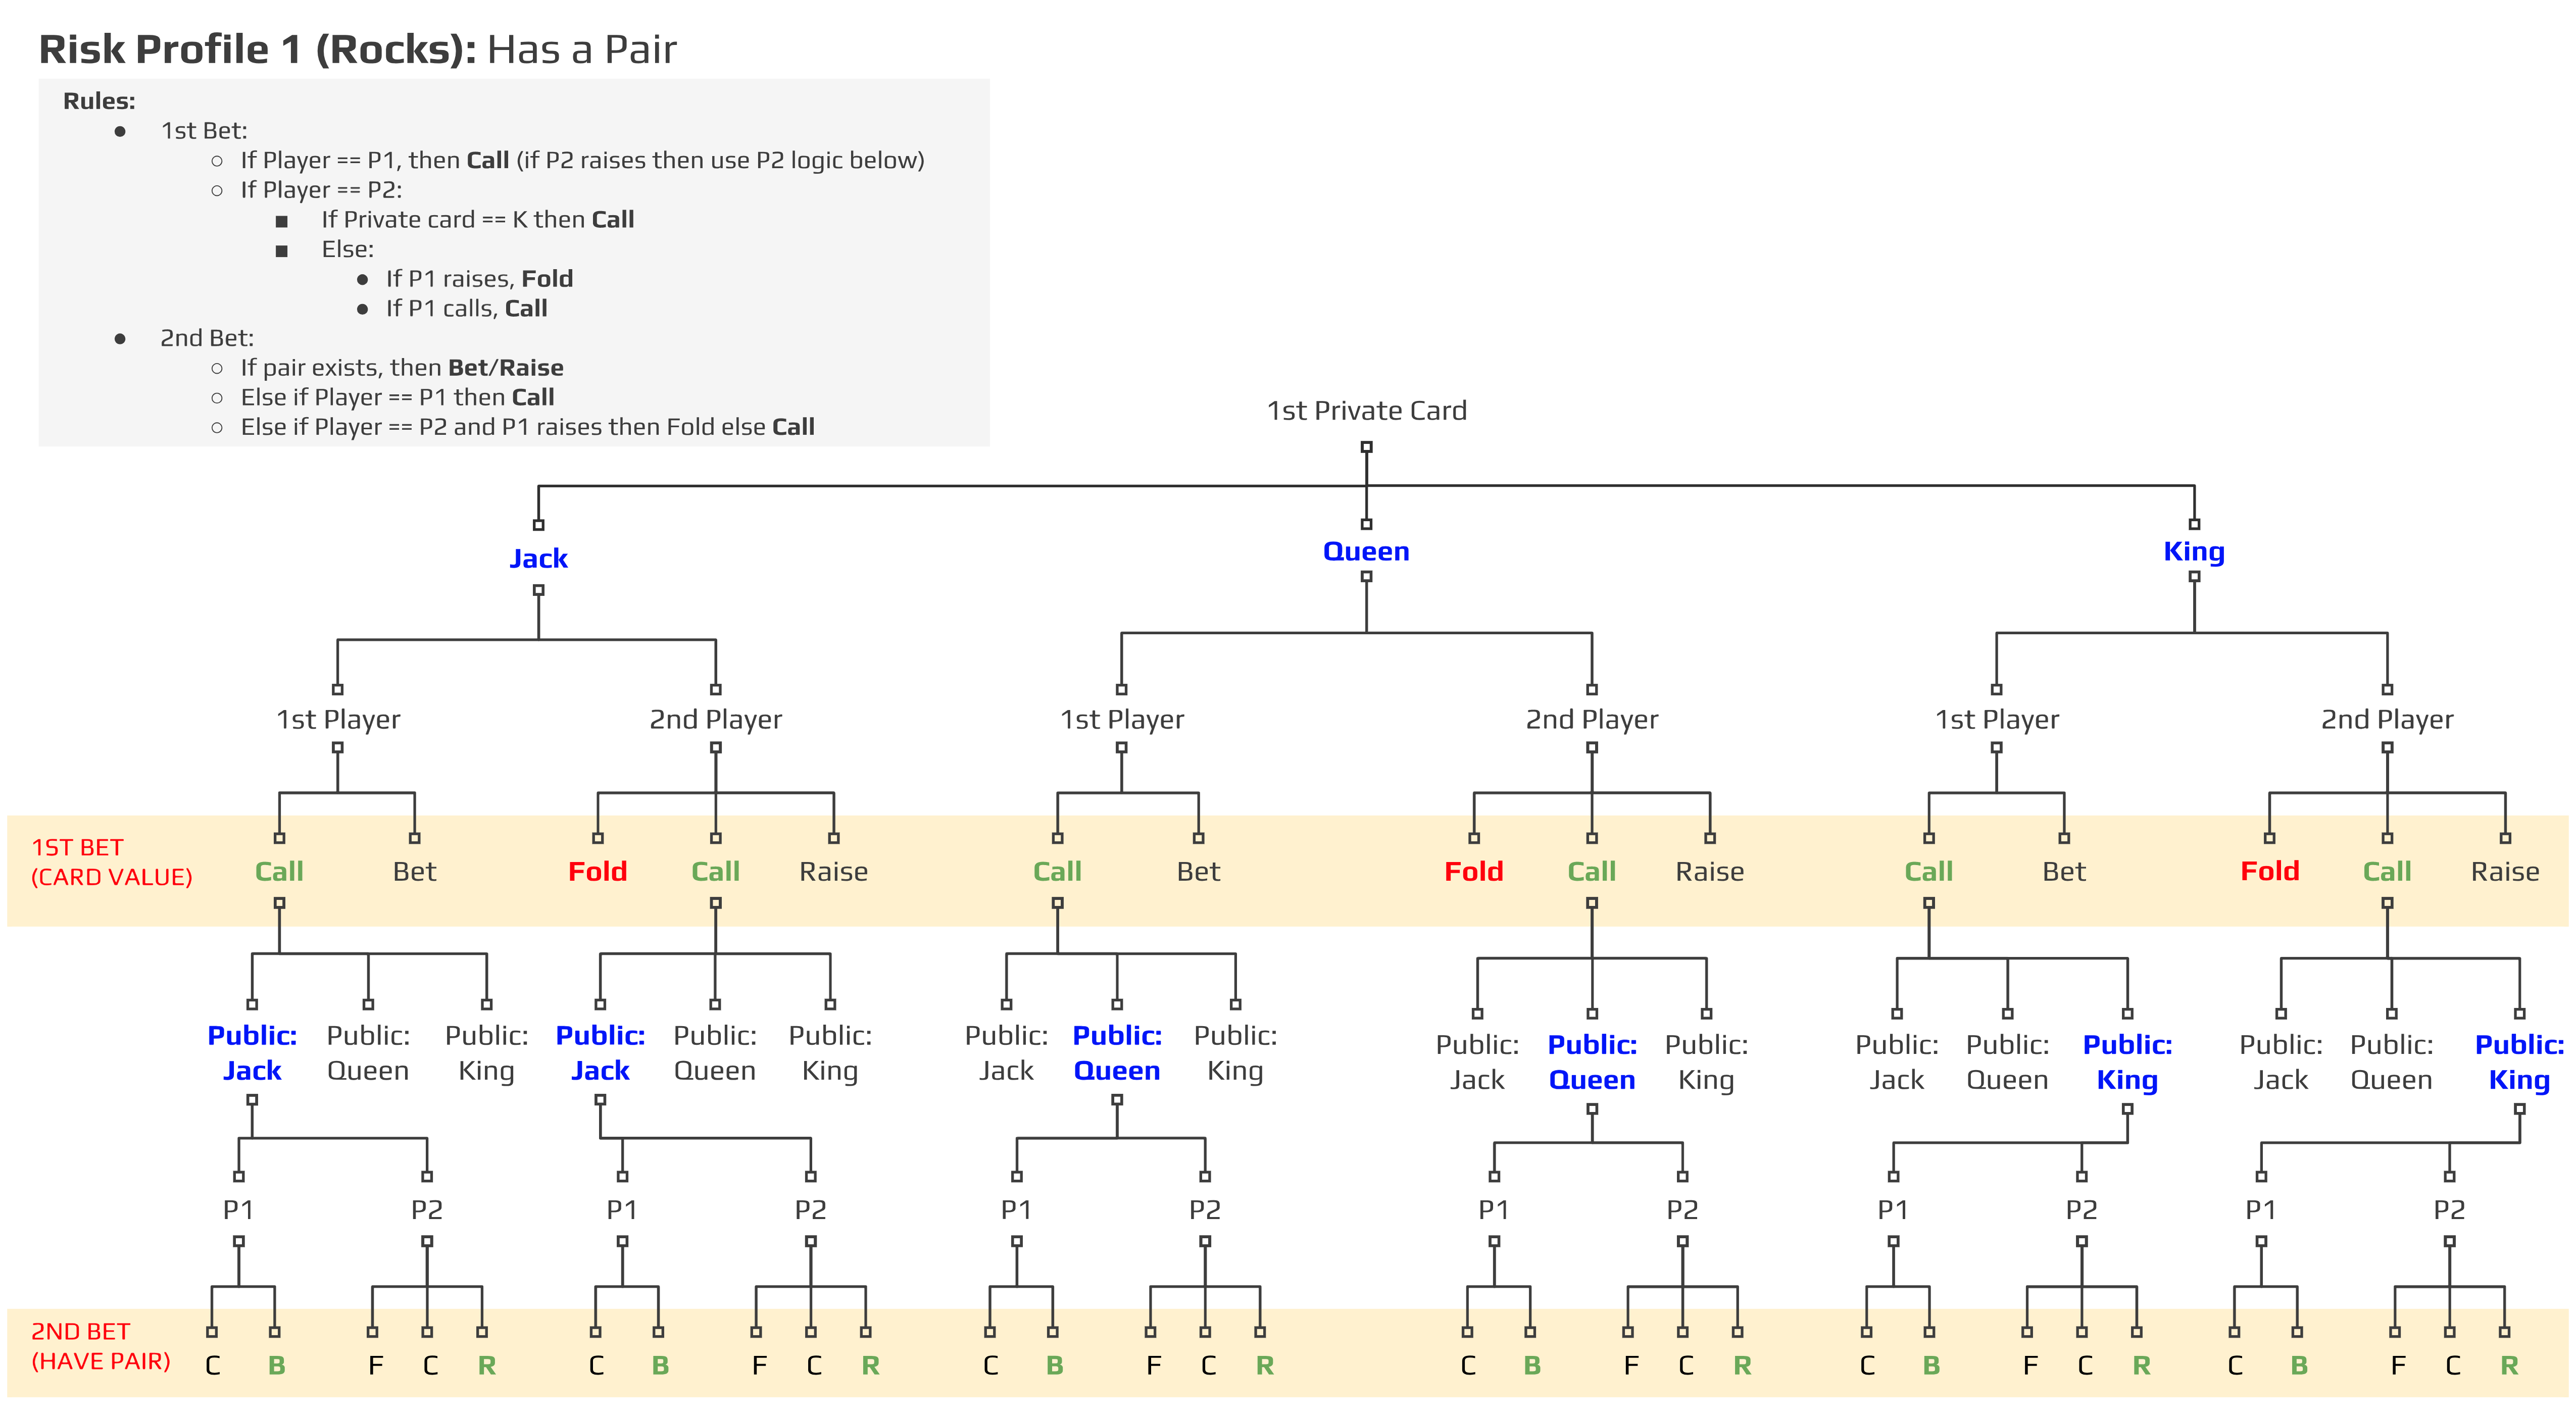
\includegraphics[width=.9\linewidth]{figures/Rocks.png}}
\end{center}
   \caption{Example of a Rocks Player Game tree in the scenario where a pair exists.}
\label{fig:short}
\end{figure*}
% rightmost sub-tree Fold should be colored in red

\subsection{Modifying DeepStack Training}
With the intent to explore the effects of a player being able to bias the training phase of DeepStack, we modified DeepStack such that it could be subject to the same training challenges of regular players by implementing a Rocks opponent playing profile that factored into generating the training/validation data set, and then trained DeepStack on this data set. To do this, we modified how the opponent’s private card ranges translated to counterfactual values influencing the opponent player’s choices. In DeepStack, this required %modifications to the \texttt{range}$\_$\texttt{generator, data}$\_$\texttt{generation} and \texttt{evaluator} classes 
to alter calculations of handling the opponent’s hand. Thus, instead of learning from self-play, the biased DeepStack learned from opponent play, where the opponent behaved like a Rocks player. Post-training, we then played this biasedly-trained DeepStack against the same playing profiles previously implemented. 

\subsection{Evaluation Criteria}
Exploitability is a typical metric used to assess performance in Leduc Hold'em. Exploitability of a strategy is defined as the measure of performance against a worst-case opponent, or distance from the Nash equilibrium strategy. Exploitability is quantified as the difference in value of the game to a player and the opponent’s payoff if the opponent plays best response. When evaluating the exploitability of our control DeepStack vs. our bias-trained DeepStack, the exploitability was 3.21 (Control) vs. 4.16 (Bias Trained). However, since our focus here is precisely to explore deviations from optimal play, this metric does not make sense to evaluate the strength of our playing profiles in this context. Instead, we simply analyze the average bankroll per hand (i.e. chips gained / lost per hand) as well as the variability in the bankroll per hand. Note that we only report average bankroll per hand instead of the standard milli-big-blinds per game (mbb/g) since there are no blinds in our game, but only an ante of 100 chips per hand. % find reference where bankroll per hand was also used for evaluating Leduc Hold'em, otherwise reviewers will comment here

\indent To evaluate the implemented biased training, we generated 10,000 examples --- one that was trained with no bias and one that was trained by the opponent playing a Rocks profile. We then trained a control DeepStack agent, with three hidden layers including two parametric rectified linear unit layers, on the original 10,000 data set and a potentially biased DeepStack (with identical neural network architecture) on the biased 10,000 data set. We then played control DeepStack and the biased DeepStack against each of the previous playing profiles.

\section{Results}
% add ack to original repo authors from previous semester, later we may setup video call with them for their feedback
%We expand upon two starter Github-repos, with code located at \href{https://github.com/rawls238/deep_learning_project}{https://github.com/rawls238/deep\_learning\_project}.  

We add to the rational DeepStack player \cite{leducdeepstack} a structure to create custom rule-based players, performance evaluation criteria, and a framework for pitting DeepStack against Libratus \cite{coms4995f17}.  We modify DeepStack's re-solver to create the players built on top of DeepStack and implement our rule-based players from scratch. %Instructions on how to play with these new players are included in the README for our project.\\
In the spirit of reproducible research we make our data, models, and code publicly available \cite{aridor19}.

\subsection{Player Risk Profile Performance}
\begin{table}
\centering
\begin{tabular}{rlll}
  \hline
 & Player & Unbiased & Biased \\ 
  \hline
  1 & Mild Adaptive Rocks & -11.4 $\pm$ 12 & 63.6 $\pm$ 28 \\ 
  2 & Passive Rocks & -43.5 $\pm$ 20 & -14.8 $\pm$ 38 \\ 
  3 & Strong Adaptive Rocks & -3.7 $\pm$ 9.4 & 53.9 $\pm$ 29 \\ 
  4 & Rocks & -1.5 $\pm$ 5.8 & 4.7 $\pm$ 18 \\ 
  5 & Random Bluffer & -53.6 $\pm$ 30 & 6 $\pm$ 34 \\ 
  6 & Smart Bluffer & -35.8 $\pm$ 24 & 23.6 $\pm$ 32 \\ 
   \hline
\end{tabular}
\caption{Average Chips Per Game on Biased vs. Unbiased Training. The table reports means and 95\% confidence intervals.}
\label{perf_results}
\end{table}

\indent Table \ref{perf_results} shows the results of our different player profiles pitted against DeepStack. %\footnote{The raw log files containing the results of each individual hand can be found in the \texttt{logs} folder of the implementation repository} 
The results in the \textit{Unbiased} column presents the results of our different player profiles against the standard trained DeepStack, which should approximate Nash Equilibrium behavior. None of our player profiles beat DeepStack by a statistically significant margin and, in fact, DeepStack beats most of the player profiles by a statistically significant margin. This was expected as all of our player profiles deliberately build in sub-optimal play to approximate the strategies used by humans and should perform worse on average. However, not all common player profiles are equally sub-optimal and certain player profiles can help a player do reasonably well against DeepStack. 

\indent While Smart Bluffer and Passive Rocks may seem like sensible player profiles, they lose substantially, on average, whereas Rocks and Strong Adaptive Rocks playing profiles only lose by a small margin. Rocks represents the most conservative player, who folds if she doesn't start with a very strong hand. It makes sense that these conservative strategies follow DeepStack closely; although they cannot play as well, by refusing to play if they don't hold strong hands, they cover their losses pretty well to not lose many chips by not getting themselves into risky situations. On the other hand, the riskiest profiles, while perhaps providing more "exciting" games, are sub-optimal in a much more exploitable way, upping the ante and therefore exposing themselves to much more risk. In conclusion, when playing against DeepStack, it is better to play safe. % rephrase this

\subsection{Biasing Training}

\indent We further explored whether it was possible to lead our sub-optimal player profiles to be able to beat DeepStack. We did this by modifying the training period to have DeepStack trained against the "Rocks" player profile and then recorded the results of gameplay across our various player profiles over one-thousand games. By training against the Rocks player profile, we expected DeepStack to still significantly exploit the weaknesses in Rocks and potentially do better than under the unbiased training against the Rocks player profile (or at least do no worse). However, we were interested to see if this would lead our other player profiles to be able to play better against DeepStack.

\indent The \textit{Biased} column in Table \ref{perf_results} shows the results of this experiment. As expected, the performance of the Rocks profile does not vary substantially between the Unbiased and Biased results. However, surprisingly, Strong Adaptive Rocks and Mild Adaptive Rocks both beat DeepStack by a statistically significant margin. The other player profiles, besides Rocks, improve their performance considerably but do not defeat DeepStack. Figure \ref{fig:strong_adaptive} shows a comparison between the distribution of chips won for the biased vs unbiased training. Note that there is significant mass in the part of the distribution where Strong Adaptive Rocks won $\geq1000$ chips for the biased training results whereas there is very little mass there under unbiased training. While the intuition behind this is not obvious, the reason is that since the biased training profile was Rocks, DeepStack failed to properly learn how to play against a range of strategies due to the conservative tendencies of the Rocks profile. This leads it to perform more poorly on ``riskier" plays, which sometimes will lead to larger bets since it will mean that the players are not folding quickly.

\indent Figure \ref{fig:strong_adaptive} shows that while the mean number of chips won for the Strong Adaptive Rocks player may have increased substantially, there may be considerably more variability in the results. Table \ref{table:sd_chips} shows that the biased training results all exhibit higher variability than the same player profiles under unbiased training. Indeed, Table \ref{table:win_rate} shows that under biased training the player profiles actually win a smaller fraction of rounds implying that they win larger pots than under unbiased training. This is consistent with the conjecture from before that the biased training technique may lead to DeepStack performing worse in "riskier" hands, since biased training did not expose DeepStack to such poker hands due to the conservative behavior of Rocks.

\begin{figure}[H]
    \centering
    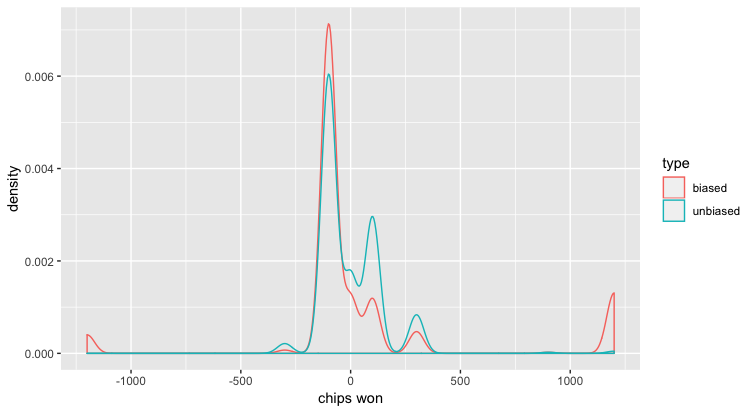
\includegraphics[scale=0.3]{figures/strong_adaptive_plot}
    \caption{Smoothed kernel density estimate of the biased vs unbiased play of strong adaptive rocks}
    \label{fig:strong_adaptive}
\end{figure}


\begin{table}
\centering
\begin{tabular}{rlll}
  \hline
 & Player & Unbiased & Biased \\ 
  \hline
1 & Mild Adaptive Rocks & 192 & 457 \\ 
  2 & Passive Rocks & 328 & 620 \\ 
  3 & Strong Adaptive Rocks & 152 & 468 \\ 
  4 & Rocks & 93.9 & 296 \\ 
  5 & Random Bluffer & 492 & 544 \\ 
  6 & Smart Bluffer & 393 & 517 \\ 
   \hline
\end{tabular}
\caption{Standard Deviation of Chips Won}
\label{table:sd_chips}
\end{table}


\begin{table}
\centering
\begin{tabular}{rlll}
  \hline
 & Player & Unbiased & Biased \\ 
  \hline
1 & Mild Adaptive Rocks & 0.371 & 0.291 \\ 
  2 & Passive Rocks & 0.455 & 0.434 \\ 
  3 & Strong Adaptive Rocks & 0.327 & 0.253 \\ 
  4 & Rocks & 0.418 & 0.331 \\ 
  5 & Random Bluffer & 0.586 & 0.466 \\ 
  6 & Smart Bluffer & 0.51 & 0.417 \\ 
   \hline
\end{tabular}
\caption{Average Win Rate (Fraction of Rounds Winning $> 0$ Chips) - Biased vs Unbiased}
\label{table:win_rate}
\end{table}

\subsection{Conclusions}

In this work we explored how traditional poker playing profiles that exhibit some degree of irrationality fared against an implementation of DeepStack in Leduc Hold'em. We showed that simple, conservative playing profiles did the best while riskier profiles lost by a substantially larger margin against an unbiased version of DeepStack. We then introduced bias in the training stage of DeepStack such that DeepStack was optimized to play against one particular player profile. 

\indent We then demonstrated that switching play to different player profiles may lead to beating the biased DeepStack on average. However, this led to increased variability in the outcome of the hands. Overall, our results are a proof of concept that point to the susceptibility of DeepStack to strategic biasing in the training stage if the training stage is learned from play against others. 

\subsection{Future Work}
% The most obvious future work is to extend our analysis to include biasing training on the other player profiles and not only the Rocks player profile. % can this be done now?
%Additionally, due to time and computational constraints all of the analysis here was done using Leduc Hold'em instead of on the more complex game of HUNL poker.
In future work we will replicate our analysis using an implementation for HUNL instead of Leduc. It would be interesting to see if the same general results hold between these two cases since computing Nash in HUNL is considerably more computationally expensive than Leduc, which would lead one to think that sophisticated agents such as DeepStack should perform even better against the irrational player profiles considered here. 

\indent Going further it would be interesting to see what would be the consequences of an "open loop" training as in Libratus in subsequent rounds of play with the same game-playing profile (constrasted with the training opponent profile). % Finally, it would be interesting to explore to a unified theory in which the weaknesses discussed here are be exploited in both perfect and imperfect information games such as games such as chess, shogi, or Go. % this raises the question why focus on imperfect information games and not perfect information games first, revise this last sentence otherwise reviewers will comment

\bibliography{bibliography}
\bibliographystyle{icml2019}
\end{document}